\usepackage[english]{babel}
\usepackage[utf8x]{inputenc}
\usepackage[T1]{fontenc}
%% Sets page size and margins
%\usepackage[a4paper,top=3cm,bottom=2cm,left=3cm,right=3cm,marginparwidth=1.75cm]{geometry}

%% Useful packages
\usepackage{amsmath,amssymb,amsthm}
\usepackage{physics}
\usepackage{mathtools}
\usepackage{tikz}
\usepackage{pgfplots}
\usepackage{graphicx}
\usepackage{xcolor}
\usepackage{tabularx}

\usepackage[colorinlistoftodos]{todonotes}

%\usetikzlibrary{backgrounds,calc}

\usetikzlibrary{shapes,arrows,backgrounds,calc}
\usepackage{color}
\usepackage{listings}
\usepackage{bm}
\usepackage{microtype} % Improves character and word spacing
\usepackage{lipsum} % Inserts dummy text
\usepackage{booktabs} % Better horizontal rules in tables
\usepackage{graphicx} % Needed to insert images into the document
\usepackage{tabularx}
\usepackage{cancel}
\definecolor{codegreen}{rgb}{0,0.6,0}
\definecolor{codegray}{rgb}{0.5,0.5,0.5}
\definecolor{codepurple}{rgb}{0.58,0,0.82}
%\definecolor{backcolour}{rgb}{0.95,0.95,0.92}
%\definecolor{backcolour}{rgb}{0.5,0.5,0.5}
%\definecolor{backcolour}{rgb}{1.0,0.937,0.859}
\definecolor{backcolour}{rgb}{1.0,1.0,1.0}
\definecolor{skyblue1}{rgb}{0.447,0.624,0.812}
\definecolor{scarletred1}{rgb}{0.937,0.561,0.561}
\definecolor{juhagray}{rgb}{0.75,0.75,0.75}
%\definecolor{backcolour}{rgb}{1.0,1.0,1.0}
 
\lstdefinestyle{mystyle}{
    backgroundcolor=\color{backcolour},   
    commentstyle=\color{codegreen},
    keywordstyle=\color{magenta},
    numberstyle=\tiny\color{codegray}, 
    stringstyle=\color{codepurple},
    basicstyle=\footnotesize,
    breakatwhitespace=false,
    frame=shadowbox,
    rulesepcolor=\color{juhagray},
    breaklines=true,                 
    captionpos=b,                    
    keepspaces=true,                 
    numbers=none,                    
    numbersep=5pt,                  
    showspaces=false,                
    showstringspaces=false,
    showtabs=false,                  
    tabsize=2
}
 
\lstset{style=mystyle}

\usepackage[american,siunitx]{circuitikz}
\usetikzlibrary{arrows,calc,positioning}


\newcommand{\Hee}{\mathcal{H}(e^{i\hat{\omega}})}
\newcommand{\Hez}{\mathcal{H}(z)}
\newcommand{\Hew}{\mathcal{H}(\omega)} 
\newcommand{\Hec}{\mathcal{H}^*\left(e^{i\hat{\omega}}\right)} 
\newcommand{\Hem}{\mathcal{H}\left(e^{-i\hat{\omega}}\right)}
%\newcommand{\He}{\mathcal{H}\left(e^{i\hat{\omega}}\right)}

\newcommand{\He}{\mathcal{H}\left(\hat{\omega}\right)}
\newcommand{\Xe}{X\left(e^{i\hat{\omega}}\right)}
\newcommand{\Xec}{X^*\left(e^{i\hat{\omega}}\right)}
%\newcommand{\Hec}{\mathcal{H}^*\left(e^{i\hat{\omega}}\right)} 
%\newcommand{\Hem}{\mathcal{H}\left(e^{-i\hat{\omega}}\right)} 
\newcommand{\Xem}{X\left(e^{-i\hat{\omega}}\right)} 

\newcommand{\mixer}[1] 
{  % #1 = name , 
\draw[thick] (#1) circle (12pt);
\draw[rotate=45,line width=0.5pt]   (#1)  +(0,-12pt) -- +(0,12pt);
\draw[rotate=-45,line width=0.5pt]  (#1)  +(0,-12pt) -- +(0,12pt);
}
\newcommand{\BPF}[2] 
{  % #1 = name , #2 = rotation angle
\begin{scope}[transform shape,rotate=#2]
\draw[thick] (#1)node[](a){} +(-12pt,-12pt) rectangle +(12pt,12pt);
\draw (a) +(-8pt,0) to[bend left] +(0,0) edge[bend right] +(8pt,0);
\draw ([yshift=5pt]a) +(-8pt,0) to[bend left] +(0,0) to[bend right] +(8pt,0);
\draw ([yshift=-5pt]a) +(-8pt,0) to[bend left] +(0,0) edge[bend right] +(8pt,0);
\draw[rotate=20] ([yshift=5pt]a) +(-4pt,0) -- +(7pt,0);
\draw[rotate=20] ([yshift=-5pt]a) +(-7pt,0) -- +(4pt,0);
\end{scope}
}
\newcommand{\LPF}[2] 
{  % #1 = name , #2 = rotation angle
\begin{scope}[transform shape,rotate=#2]
\draw[thick] (#1)node[](a) {\footnotesize{$\mathcal{H}(\omega)$}} +(-12pt,-12pt) rectangle +(12pt,12pt);
\end{scope}
}

\newcommand{\hangp}[1]{\makebox[0pt][r]{(}#1\makebox[0pt][l]{)}} % New command to create parentheses around text in tables which take up no horizontal space - this improves column spacing
\newcommand{\hangstar}{\makebox[0pt][l]{*}} % New command to create asterisks in tables which take up no horizontal space - this improves column spacing

\tikzset{ar/.style={-latex,shorten >=-1pt, shorten <=-1pt}}
\usetikzlibrary{shapes,arrows}


\hypersetup{colorlinks} % Comment this line if you don't wish to have colored links


\setkeys{Gin}{width=\linewidth,totalheight=\textheight,keepaspectratio} % Improves figure scaling

\usepackage{fancyvrb} % Allows customization of verbatim environments
\fvset{fontsize=\normalsize} % The font size of all verbatim text can be changed here


\usepackage{xspace} % Used for printing a trailing space better than using a tilde (~) using the \xspace command

\newcommand{\monthyear}{\ifcase\month\or January\or February\or March\or April\or May\or June\or July\or August\or September\or October\or November\or December\fi\space\number\year} % A command to print the current month and year

\newcommand{\openepigraph}[2]{ % This block sets up a command for printing an epigraph with 2 arguments - the quote and the author
\begin{fullwidth}
\sffamily\large
\begin{doublespace}
\noindent\allcaps{#1}\\ % The quote
\noindent\allcaps{#2} % The author
\end{doublespace}
\end{fullwidth}
}
\usetikzlibrary{shapes,snakes}

\newcommand\Hiw{\mathcal{H}(\omega)}

\tikzset{%
    dimen/.style={|-|,>=latex,thin,every rectangle node/.style={fill=white,midway,font=\sffamily}},
}

\pgfplotsset{
    dirac/.style={
        mark=triangle*,
        mark options={scale=2},
        ycomb,
        scatter,
        visualization depends on={y/abs(y)-1 \as \sign},
        scatter/@pre marker code/.code={\scope[rotate=90*\sign,yshift=-2pt]}
    }
}

\tikzstyle{int}=[draw, minimum size=2em]
\tikzstyle{init} = [pin edge={to-,thin,black}]

 
\newcommand{\spop}[1][\cdot]{\mathcal{T}\left\{#1\right\}}
\newcommand{\spopb}{\mathcal{T}}

\newcommand{\blankpage}{\newpage\hbox{}\thispagestyle{empty}\newpage} % Command to insert a blank page

\usepackage{imakeidx} % Used to generate the index
\usepackage{hyperref}
\makeindex % Generate the index which is printed at the end of the document

%----------------------------------------------------------------------------------------
%	BOOK META-INFORMATION
%----------------------------------------------------------------------------------------
\author{Juha Vierinen} % Author
\publisher{University of Troms\o{}} % Publisher

%----------------------------------------------------------------------------------------


\newsavebox{\titleimage}
\savebox{\titleimage}{
\centering{
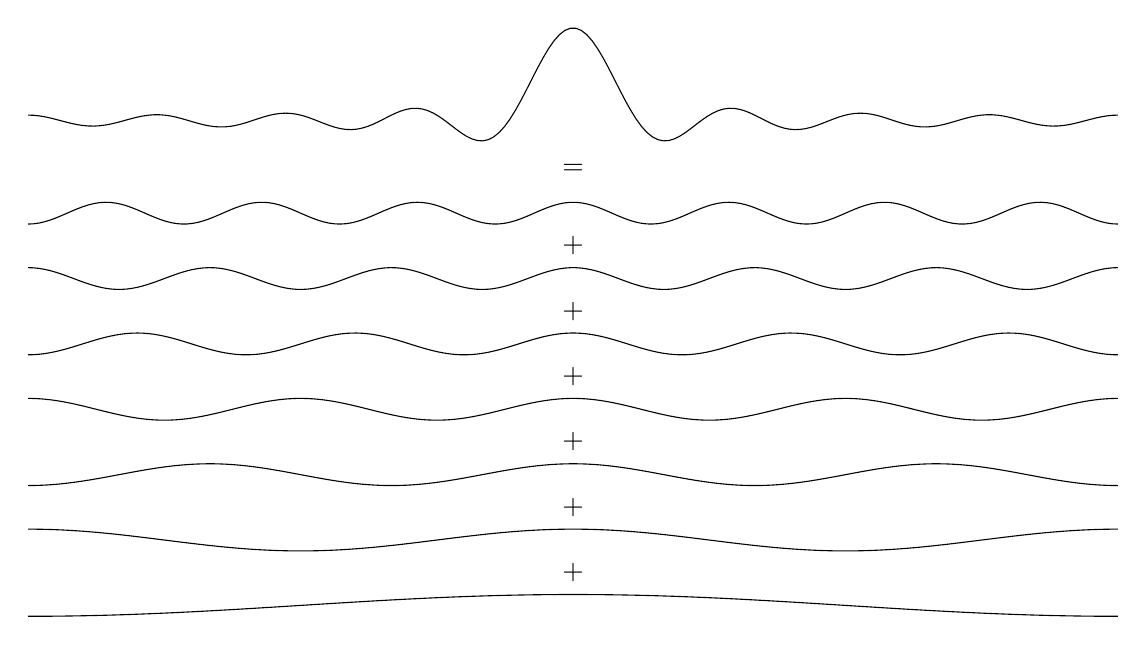
\begin{tikzpicture}
% \begin{pgfinterruptboundingbox}
\begin{axis}[width=1.5\textwidth, height=30em,
%	title={Discrete-time signal},
	axis x line=none,
	axis y line=none
]
\addplot[domain=-100:100,samples=200] {27+
                                       cos( deg(2*3.1415*0.01*0.5*x))+
                                       cos( deg(2*3.1415*0.01*0.5*2*x) )+
                                       cos( deg(2*3.1415*0.01*0.5*3*x) )+
                                       cos( deg(2*3.1415*0.01*0.5*4*x) )+
                                       cos( deg(2*3.1415*0.01*0.5*5*x) )+
                                       cos( deg(2*3.1415*0.01*0.5*6*x) )+
                                       cos( deg(2*3.1415*0.01*0.5*7*x) )+
                                       cos( deg(2*3.1415*0.01*0.5*8*x) ) };

\node at (axis cs:0,22) {$=$};
\node at (axis cs:0,15) {$+$};
\node at (axis cs:0,9) {$+$};
\node at (axis cs:0,3) {$+$};
\node at (axis cs:0,-3) {$+$};
\node at (axis cs:0,-9) {$+$};
\node at (axis cs:0,-15) {$+$};
                                      
\addplot[domain=-100:100,samples=200] {-18+cos( deg(2*3.1415*0.01*0.5*x) ) };
\addplot[domain=-100:100,samples=200] {-12+cos( deg(2*3.1415*0.01*0.5*2*x) ) };
\addplot[domain=-100:100,samples=200] {-6+cos( deg(2*3.1415*0.01*0.5*3*x) ) };
\addplot[domain=-100:100,samples=200] {0+cos( deg(2*3.1415*0.01*0.5*4*x) ) };
\addplot[domain=-100:100,samples=200] {6+cos( deg(2*3.1415*0.01*0.5*5*x) ) };
\addplot[domain=-100:100,samples=200] {12+cos( deg(2*3.1415*0.01*0.5*6*x) ) };
\addplot[domain=-100:100,samples=200] {18+cos( deg(2*3.1415*0.01*0.5*7*x) ) };
\end{axis}
%\end{pgfinterruptboundingbox}
%\draw[use as bounding box] ([xshift=0cm,yshift=0cm]current axis.south west) 
%    rectangle ([xshift=0cm,yshift=0cm]current axis.north east);
\end{tikzpicture}
}
}

\title[Signal processing]{%
  \setlength{\parindent}{0pt}%
  Signal processing\par \vspace{1cm}
    \usebox{\titleimage}
  }
  
\author{Juha Vierinen, J\o{}rn Olav Jensen}
\date{Fall 2022}
